
\documentclass{article}[12pt,a4paper]
\usepackage{graphicx}
\usepackage{geometry}
\usepackage{tikz}
\usetikzlibrary{calc}
\linespread{1.6}
\usepackage{setspace}
\renewcommand{\familydefault}{\rmdefault}
\begin{document}
\begin{titlepage}
    \begin{singlespacing}
    \begin{tikzpicture}[remember picture, overlay]
    %   \draw[line width = 1pt] ($(current page.north west) + (2em,-2em)$) rectangle ($(current page.south east) + (-2em,2em)$);
    \end{tikzpicture}

    \centering
    \vspace{-3em}
    {\Large\textbf{IR Project Proposal Report}}\\
    \vspace{1em}
    On\\
    \vspace{1em}
    {\Huge \textbf{Person Re-Identification using Deep Learning Techniques}}\\
    \vspace{2em}
    {\LARGE \bfseries Submitted by}\\
    \vspace{2em}
    {\Large \emph{\textbf{15IT137.  Revanth B S}}}\\
    \vspace{0.5em}
    {\Large \emph{\textbf{15IT203.  Akshay U Prabhu}}}\\
    \vspace{0.5em}
    {\Large \emph{\textbf{15IT252.  Hafeez Ali A}}}\\
    \vspace{2em}
    {\Large Under the Guidance of}\\
    \vspace{2em}
    {\Large \textbf{Dr. Sowmya Kamath S}}\\
    \vspace{2em}
    {\Large \textbf{Dept. of Information Technology,}}\\
    \vspace{1em}
    {\Large \textbf{NITK, Surathkal}}\\
    \vspace{2.5em}
    {\Large \textbf{Date of Submission: 1st May 2018}}\\
    \vspace{1em}
    \begin{figure}[!ht]
        \centering
        
\includegraphics{nitk-logo.png}
    \end{figure}
    \vspace{1em}
    {\Large \bfseries Department of Information Technology}\\
    \vspace{0.5em}
    {\Large \bfseries National Institute of Technology Karnataka, Surathkal.}\\
    \vspace{1em}
    {\Large \bfseries 2017-2018}
    
    \end{singlespacing}
\end{titlepage}

\pagenumbering{roman}
\section*{Abstract}
\addcontentsline{toc}{section}{Abstract}

Person re-identification is the process of identifying an individual as a person from an earlier scenario. The primary challenge of person re-identification is the ability to recognize the identity of a person under varying conditions of light, line of sight, pose, occlusions etc. A deep learning approach to the problem requires the deep learning model to be able to learn features that are invariant under the about mentioned perturbations. We implement a convolutional neural network based architecture used in this paper\cite{base_paper} which tries to classify a person into any of the classes of recognized individuals. We show that this implementation performs poorly for datasets when very few same class samples are available. We propose a model based on siamese neural networks to tackle the problem of insufficient data. This model takes a pair of images as output and predicts whether the pair contains images of the same person or two different persons. During training the model tries to learn features which improves intra-class similarity and reduces inter-class similarity. Once the network has been tuned we can use the discriminative features generated by the network not just on new images but also on entirely different classes of unknown datasets. We will show that the featured vectors produced by the trained model generalizes well on new datasets.

\newpage
\section*{Declaration}
\addcontentsline{toc}{section}{Declaration}

We hereby declare that the mini project entitled "Person Re-Identification using Deep Learning Techniques", is a record of an original work done by us at the Department of Information Technology, National Institute of Technology Karnataka, Surathkal, during the academic semester of Jan - May 2018 in partial fulfillment of the requirements for the award of the degree of Bachelor of Technology in Information Technology, at NITK Surathkal under the guidance of Dr. Sowmya Kamath S.

\begin{enumerate}
    \item Revanth B S
    \item Akshay U Prabhu
    \item Hafeez Ali A
\end{enumerate}

\vspace{3em}
Place:

Date:

\newpage
\section*{Certificate}
\addcontentsline{toc}{section}{Certificate}

This is to certify that the Mini Project entitled "Person Re-Identification using Deep Learning Techniques" is a bonafide work carried out under my guidance by:

\begin{enumerate}
    \item Revanth  S
    \item Akshay U Prabhu
    \item Hafeez Ali A
\end{enumerate}

students of VI Sem B.Tech(IT) at the Department of Information Technology, National Institute of Technology Karnataka, Surathkal,  during the academic semester of Jan - May 2018 in partial fulfillment of the requirements for the award of the degree of Bachelor of Technology, at NITK Surathkal.

\vspace{3em}
Place:

Date:\hfill (Sowmya Kamath)


\newpage
\tableofcontents
\newpage
\listoffigures
\newpage
\listoftables
\thispagestyle{empty}
\newpage
\pagenumbering{arabic}

\section{Introduction}


Person re-identification is the task of recognizing an individual who has previously been observed over a camera network. It is a challenging computer vision task that can provide useful tools for many security applications of video-surveillance, e.g., on-line tracking of individuals over different, non-overlapping cameras, and off-line retrieval of the video sequences containing an individual of interest, whose image is given as a query. Clothing appearance is the most widely used cue, since the low image resolution and the variety of poses typical of video-surveillance settings make face recognition ineffective. State-of-the-art re-identification methods build descriptors of clothing appearance often based on a subdivision of the body into parts, and extract a set of low-level features from each part, like SIFT points, or small image patches.

The problem of person re-identification can be divided into three parts; person detection, person tracking, person retrieval. The part we are interested about is the third part, that is person retrieval. This part involves comparing a person currently being tracked with the ones that are already identified, hoping to find a match. The challenge with image re-identification is to recognize the identity of a person under different lighting conditions, occlusions, camera viewpoints. This proves to be a difficult task when the datasets contain very few low resolution images of different camera viewpoints of the same person.

Previous approaches rely on Principle Component Analysis to extract important features and reduce dimension. Then the recovered features are fine tuned using a neural network model. Several other approaches have been proposed which use features produced using LBP and SIFT techniques. Most of these methods assume that test and training samples are produced under same external conditions like light and background. This assumption is not true under most of the real world circumstances.

We implement a convolutional neural network which tries retrieve, given a sample image of a person, all the images of that person in the dataset. This method produces poor results on small and medium sized datasets due to insufficient same class images. To solve this we have used a Siamese neural network which takes as input, a pair of images either belonging to the same class or different classes, and tries to predict whether the pair of images belong to the same class or different classes. During the learning process the network learns features that effectively discriminate interclass images and that are indifferent towards intraclass features. We can use this feature vector generated by the model and find the most similar images using any of the similarity measures like cosine distance, l1 distance, l2 distance, etc. 

\section{Literature Survey}

\subsection{Related Work}
Person re-identification has seen a lot of research in the last few years. This can be attributed to rising safety and security concerns and increase in the number of surveillance cameras at various locations. With the establishment of large-scale video surveillance network in place, the task of re-identifying images has been approached using a variety of effective strategies. The primary challenge of person re-identification is the ability to recognize the identity of a person under varying conditions of light, line of sight, pose, occlusions etc.

Many excellent methods have be developed to tackle the task of person re-identification. For example, Liao et al. \cite{LOMO} improved on the KISSME method by learning a discriminant low dimensional vector based on LOMO features. Li at al. \cite{LADF} proposed the learning of Locally Adaptive Decision Functions(LADF) for person verification. This model uses a distance metric with a dynamic threshold into Mahalanobis distance to measure similarity. Prosser et al. \cite{RankSVM} viewed the person re-identification problem as a ranking problem, using RankSVM to do the same.

Several other classification techniques could be used for the task of image re-identification.For Example Koch, Zemel, Salakhutdinov Siamese Neural Networks for One-shot Image Recognition \cite{siamese}. Wang et al. use convolutional neural networks to extract discriminant features and use transfer learning to re-identify a person by ranking images based on decreasing similarity of the feature vectors obtained from the corresponding pairs of images.
\newpage

\subsection{Identified Gaps}
\begin{enumerate}
\item Most of these methods assume that test and training samples are produced under same external conditions like light and background. This assumption is not true under most real world circumstances.
\item The problem with standard deep learning based approaches is the inability to generalize for small to medium size datasets when the number of interclass images are very low.
\end{enumerate}

\subsection{Problem Statement}
Person Re-identification using Deep learning Techniques.
\subsection{Objectives}
\begin{enumerate}
    \item To implement the model proposed in the title Person Re-identification using deep features and transfer learning.
    \item To analyse the learning process of the implemented model to find why the model doesn't generalize well on small datasets.
    \item To implement a Siamese neural network for person re-identification to extract discriminating features from very few number of intraclass images.
    \item To compare and analyse the results of the two models.
\end{enumerate}
\newpage
\section{Methodology}
\subsection{Base Model}
In the paper\cite{base_paper} we have chosen to implement, they have used a model called Feature Net based on VGG16 architecture which has achieved state-of-the-art performance on ImageNet dateset. Detailed structure of the model is listed in Table 1. The Feature Net model uses VGG16 model with batch normalization.  Batch normalization helps in accelerating the convergence process. BN indicates a Batch Normalization layer. Conv indicates a convolutional layer. FC represents a fully connected layer. ReLU represents the Rectified Linear Unit activation function. The model contains 16 convolutional layers. first two Conv layers contain 64 filter, next two Conv layers contain 128, 256 filters are present in the next three Conv layers.  The last six layers contain 512 filters. Second last fully connected layer contains 64 nodes, which is connected to N nodes in the net fully connected layer, where N represents the number of test classes. The gradient descent algorithm used to achieve convergence is RMSProp and cosine similarity is used to find the similarity between feature vectors generated by the model.
\vfill

\begin{table}[h]
\begin{center}
\begin{tabular}{|l|l|l|l|}
\hline
name & & Kernel size/ stride/ pad & output size \\
\hline
input & & & 160 x 60 x 3 \\
\hline
conv1 & (Conv + BN + ReLU) * 2 & 3/1/1 & 64 x 160 x 60 \\
\hline
& Maxpool1 & 2/2 & 64 x 80 x 30 \\
\hline
conv2 & (Conv + BN + ReLU) * 2 & 3/1/1 & 128 x 80 x 30 \\
\hline
& Maxpool2 & 2/2 & 128 x 40 x 15 \\
\hline
conv3 & (Conv + BN + ReLU) * 3 & 3/1/1 & 256 x 40 x 15 \\
\hline
& Maxpool3 & 2/2 & 256 x 20 x 7  \\
\hline
conv4 & (Conv + BN + ReLU) * 6 & 3/1/1 & 512 x 20 x 7\\
\hline
& Maxpool4 & 2/2 & 512 x 10 x 4 \\
\hline
fc5 & FC + ReLU & & 64 \\
\hline
fc5 & FC + ReLU & & N \\
\hline
\end{tabular}
\caption{Detailed architecture of Feature Net}
\end{center}
\end{table}


\begin{figure}\hspace{6em}
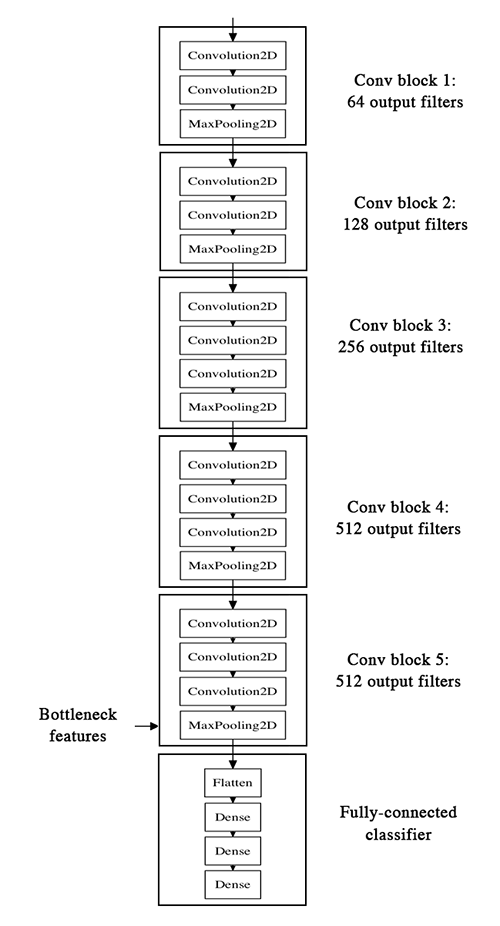
\includegraphics[scale=0.6]{vgg16}
\caption{Architecture of CNN model}
\centering
\end{figure}
\newpage

\subsection{Siamese Model}
We chose to implement a Siamese model for the problem of image re-identification because Siamese models tend to generalize well for unknown classes even when very few samples are available for each class. We used a simple 2 layer convolutional neural network with max pooling, ReLU activation as a base common network. We group the input images into positive pairs(containing images of same class) and network pairs(containing images of different classes) and label them 1 and 0 respectively. We then pass the input pairs to the base neural network to obtain a pair of feature vectors. We then measure the similarity between the two images by measuring the euclidean distance between the two feature vectors. The output is passed to a binary categorical cross entropy function to calculate the loss. Once the model is trained, given an image of a person, we calculate its feature vector using the trained network; find the similarity between this vector and the feature vectors of all the images in the test dataset. Rank the images in the decrease order of similarity and display the images with highest similarity.
\vspace{3em}
\begin{table}[h]
\begin{center}
\begin{tabular}{|l|l|l|l|}
\hline
name & & Kernel size/ stride/ pad & output size \\
\hline
input & & & 160 x 60 x 3 \\
\hline
conv1 & (Conv + BN + ReLU) * 2 & 3/1/1 & 64 x 160 x 60 \\
\hline
& Maxpool1 & 2/2 & 64 x 80 x 30 \\
\hline
conv2 & (Conv + BN + ReLU) * 2 & 3/1/1 & 128 x 80 x 30 \\
\hline
& Maxpool2 & 2/2 & 128 x 40 x 15 \\
\hline
fc5 & FC + ReLU & & 256 \\
\hline
fc5 & FC + ReLU & & 4096 \\
\hline
l2 distance & Lambda 7 & & 1 \\
\hline
\end{tabular}
\caption{Detailed architecture of Siamese Network}
\end{center}
\end{table}

\begin{figure}\hspace{6em}
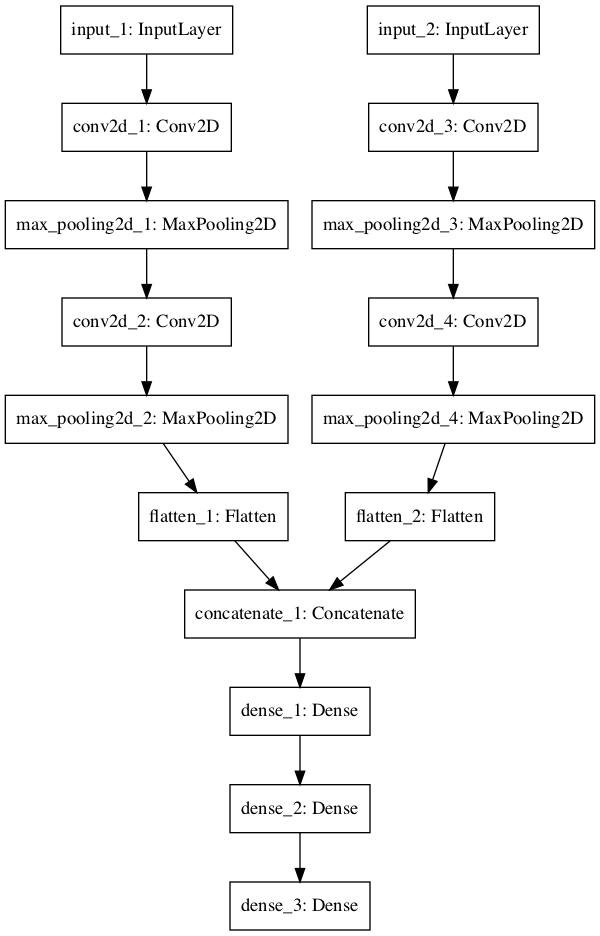
\includegraphics[scale=0.5]{siamese}
\caption{Architecture of Siamese model}
\centering
\end{figure}
\newpage

\section{Work Done and Individual Contribution}
For the base model dataset used for training and testing is the CUHK01 dataset. This dataset contains image of 971 persons taken from four different cameras to give a total of 3884 images. We divided the dataset into 3 parts training, validation and testing using 70 : 10 : 20 split. 
Preprocessing of the data involved labelling the images and resize them to fit the input shape of the designed neural network. Once the preprocessing is done the image was trained on all the images with a batch size of 64 for 500 epochs. Then accuracy of validation and testing data were calculated. The programming was done in python using Keras library with Tensorflow backend. Metrics like loss, validation loss,  accuracy, validation accuracy were calculated after every epoch using keras callback module. The model weights were saved after every epoch.

We used the same dataset for the Siamese network. Preprocessing for Siamese model included preprocessing done for the base model followed by creating positive and negative pairs and corresponding labels. Once the preprocessing is done the two inputs are given to the two input layers of the model. The output vectors form the base common model is retrieved. Euclidean distance is calculated between the two vectors. The output is given to a binary cross entropy function. Once the model is trained on the training dataset. The feature  vector generated by the common base model is used to measure similarity between images. Given an new image, we first calculate the feature vector for the image; then we measure the euclidean distance between this feature vector and the feature vectors of all the images. The results are ranked in increasing order of distance. First few images are displayed as results. accuracy is calculated by checking how many of the retrieved images belong to the same class.
\begin{table}[b]
    \centering
    \begin{tabular}{|c|c|} \hline
         Member & Individual Contribution \\ \hline
         Revanth B S & Implementation of Siamese model for person reidentification  \\ \hline
         Akshay U Prabhu & Implementation of CNN model for person reidentification \\ \hline
         Hafeez Ali A & Viola Jones Object Detection, Data preprocessing,  Triplet loss calculation \\ \hline
    \end{tabular}
    \caption{Individual Contribution of members}
    \label{tab:my_label}
\end{table}
\newpage
\section{Results and Analysis}
We used CUHK01 dataset for measuring the accuracy of the model. The data set contains images of 971 different person taken from four different cameras to provide a total 3884 images.
We divided the dataset into 3 parts training, validation and testing using 70 : 10 : 20 split. Preprocessing of the data involved labelling the images and resize them to fit the input shape of the designed neural network. Once the preprocessing is done the image was trained on all the images with a batch size of 64 for 500 epochs. Then accuracy of validation and testing data were calculated. The programming was done in python using Keras library with Tensorflow backend. We used the same dataset for the Siamese network. Preprocessing for Siamese model included preprocessing done for the base model followed by creating positive and negative pairs and corresponding labels. Once the preprocessing is done the two inputs are given to the two input layers of the model. The output vectors form the base common model is retrieved. Euclidean distance is calculated between the two vectors. The output is given to a binary cross entropy function. Once the model is trained on the training dataset. Metrics like loss, validation loss,  accuracy, validation accuracy were calculated after every epoch using keras callback module. The model weights were saved after every epoch. 
The training and testing accuracy obtained are listed in the Table 3 below. 

\begin{table}[b]
    \centering
    \begin{tabular}{| c | c | c | c |} \hline
         Datasets & Model & Training & Testing \\ \hline
         CUHK01 & base model & 67.23 & 56.987 \\ \hline
         CUHK03 & siamese model & 71.33 & 58.192 \\ \hline
    \end{tabular}
    \caption{Comparison of base model and siamese model}
    \label{tab:my_label}
\end{table}
\vspace{3em}
We can see that the siamese model performs slightly better to the base model which uses VGG16 architecture. So we can say that Siamese model is better at learning features which are better at distinguishing different class images.

\newpage
\begin{thebibliography}{1}
\addcontentsline{toc}{section}{References}
    
\bibitem{base_paper} Person Re-identification with Deep Features and Transfer Learning
Shengke Wang1, Shan Wu1, Lianghua Duan1, Changyin Yu1, Yujuan Sun2, Junyu Dong1
\bibitem{LOMO} Person Re-identification by Local Maximal Occurrence
Representation and Metric Learning
Shengcai Liao, Yang Hu, Xiangyu Zhu, and Stan Z. Li
\bibitem{LADF} Learning Locally-Adaptive Decision Functions for Person Verification
Zhen Li, Shiyu Chang, Feng Liang, Thomas S. Huang, Liangliang Cao, John R. Smith
\bibitem{RankSVM} Person Re-Identification by Support Vector Ranking
Wei-Shi Zheng, Shaogang Gong, Tao Xiang
\bibitem{siamese} Siamese Neural Networks for One-shot Image Recognition
Gregory Koch, Richard Zemel, Ruslan Salakhutdinov
\end{thebibliography}
\end{document}